\section{Interpretation}
\label{sec:vergleich}
Die Ergebnisse verdeutlichen, dass die Servicequalität einen starken Einfluss auf die Nutzerzufriedenheit und die Nutzerzufriedenheit wiederum einen starken Einfluss auf den Net Benefit hat (H2 und H3). Die Systemqualität hat hingegen keinen signifikanten Einfluss auf die Nutzerzufriedenheit (H1). Der Servicequalität konnte ebenfalls kein direkter Einfluss auf den Net Benefit nachgewiesen werden, allerdings verfügt sie über die Nutzerzufriedenheit über einen indirekten Einfluss auf den Net Benefit. 
	

Limitations
Ein MOOC ist meist Die Studie ist begrenzt auf einen MOOC der Leuphana Digital School, mit einer für einen MOOC geringen 

Samplegröße
Limitation der Konstrukte

Ausblick
Ergänzung 



  hingegen nicht bestätigt werden. Die Systemqualität konnte dagegen kein signifikanter Einfluss auf die Nutzerzufriedenheit attestiert werden. Au 
\todo consistency at large. 
Hohe Dropout Raten bei MOOCS. Besonderheiten von MOOC auflisten: 


The story of MOOCs is not going to be told with conventional statistics borrowed from brick-and-mortar classroom models. Rather, our research describes an emerging learning ecosystem, one where enrollment can be casual and nonbinding, learning happens asynchronously, and registrants come from all countries in the world, with diverse intentions and patterns of learning. The metrics we choose should respect their intentions and encourage their learning.\parencite{reich2014tricky}


\begin{figure}[h]
\centering
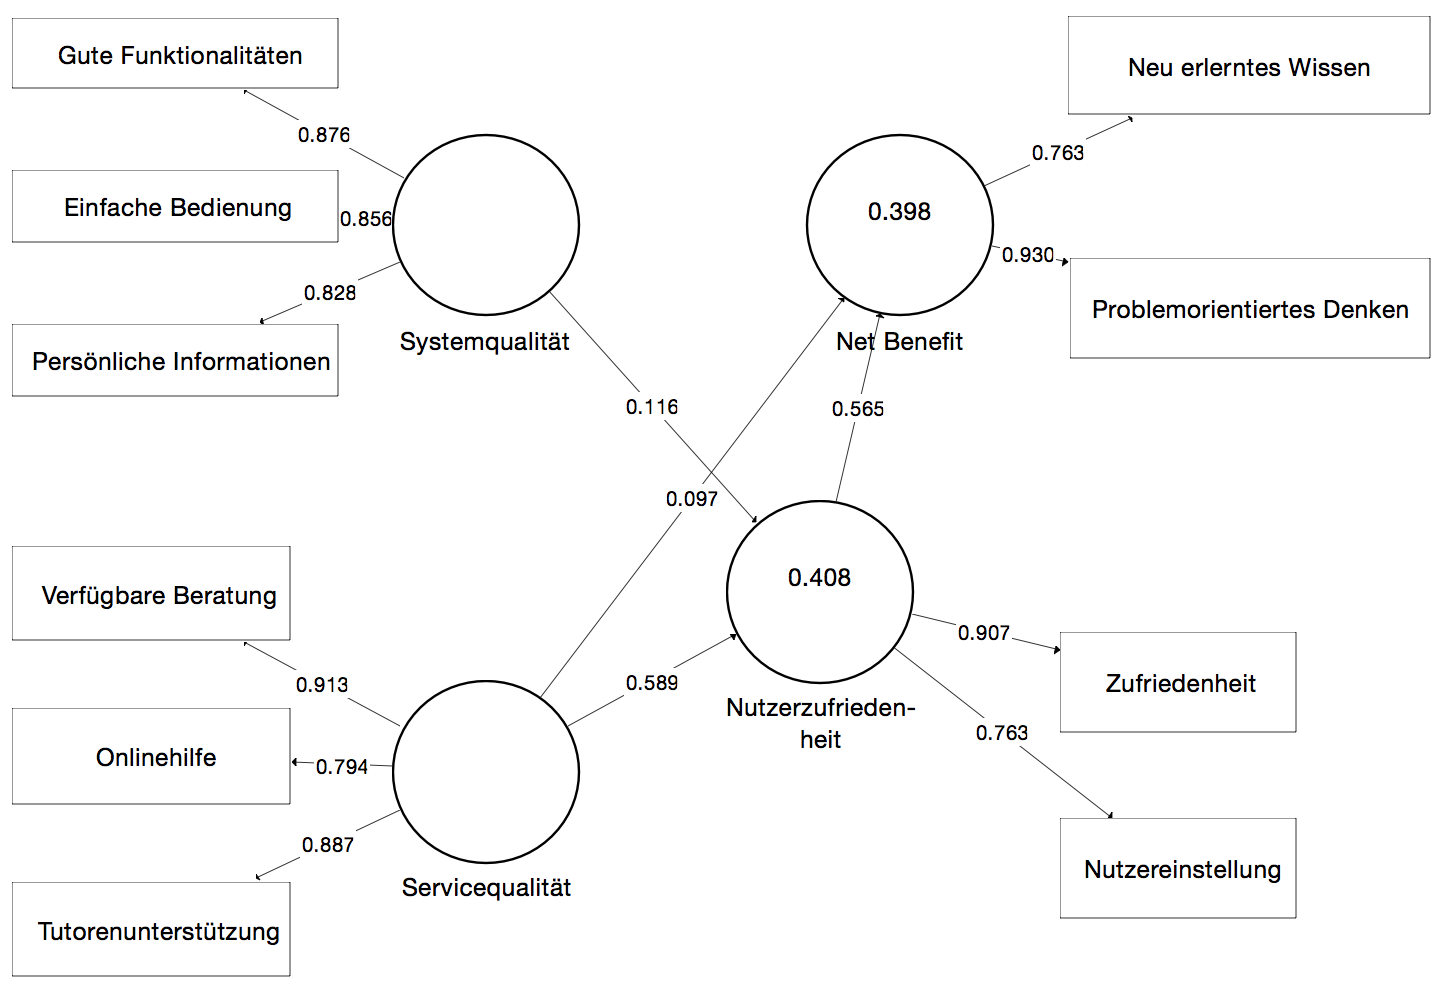
\includegraphics[width=1\textwidth]{Grafiken/pls_bw_3.png}
\caption{PLS Modellergebnisse}
\label{PLS Modellergebnisse}
\end{figure}